\chapter{Results and Discussion}

\section{Identification of Significant Features}

This project employs unsupervised learning, specifically a K-means clustering algorithm, to identify the most relevant features for describing pain. This is done by generating clusters, where K is the number defined by the user for the quantity of centroids \cite{Ikotun2023}. The clustering technique partitions data according to specific distance metrics, and `cityblock' was chosen because of the way centroids are computed, that is, as the component-wise median of points in each cluster. Besides this, this metric measures the sum of absolute differences between data point coordinates, according to Equation \ref{eq:3} and assigns points to clusters based on this distance \cite{Ricken2023}.

\begin{equation} \label{eq:3}
d(x,y)=\sum_{i=1}^{n}\left| x_i-y_i \right|
\end{equation}

This clustering algorithm was applied to every possible pair of features, with the number of centroids set to $K=2$, using data from the second baseline and from the pain stimulation phase of the fifteen participants. It's important to mention that this analysis was firstly done with the first baseline but, comparing both options, the results were better using the second one, which may stem from the influence of the emotional stimuli in the pain felt by the participants.

The result of clustering applied to two features -- the medians of the median of the S peak amplitude (x-axis) and of the median of the R offset amplitude (y-axis) -- is displayed in Figure \ref{fig:cluster} (right). In it, the two clusters defined by the algorithm can be seen, as well as X's in the position of the clusters' centroids.
For comparison, scattering graphics were plotted for each two features, as can be seen in Figure \ref{fig:cluster} (left). The incorrect matches made by the clustering algorithm are circled in black.

%\begin{figure}[h!]
    %\centering
    %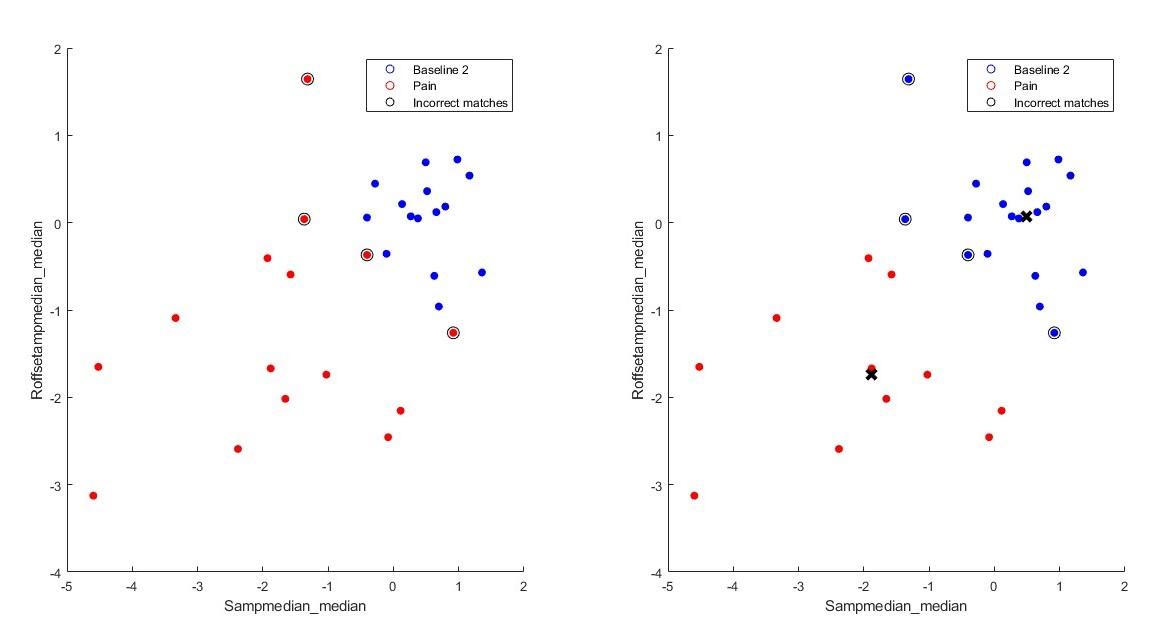
\includegraphics[width=1.0\textwidth]{cluster.jpg}
    %\caption{Scattering plot with data from baseline 2 and pain (left), and with the result of K-means clustering (right), when comparing the Roffsetampmedian\_median and Sampmedian\_median.}
    %\label{fig:cluster}
%\end{figure}

\pagebreak
Only the pairs of features where more than 80\% of the observations were correctly predicted were considered valid. A network map illustrating these pairs was plotted in Figure \ref{fig:map80}. In this map, each circle corresponds to a feature, while the lines connecting them showcase the combinations that met the accuracy threshold. Additionally, the size of the circles is proportional to how many times that specific feature, paired with another, contributed to successful clustering. These results suggest that these five features, Roffsetampmedian\_median, Sampmedian\_median, Entropydb4Approx\_median, and Entropydb9Approx\_median, when paired with each other, are the most effective in distinguishing pain from no pain. A possible takeaway from this result is that pain affects the intensity of ventricular polarization, since the S wave and R offset are related to it. Regarding the entropy, pain affects it the most in the low frequencies of the \ac{ecg} signal, for both the db4 and db9 wavelets. This might entail that the QRS complex, as concluded before, and the fluctuations of the signal also affect pain.





\begin{figure}[h!]
    \centering
    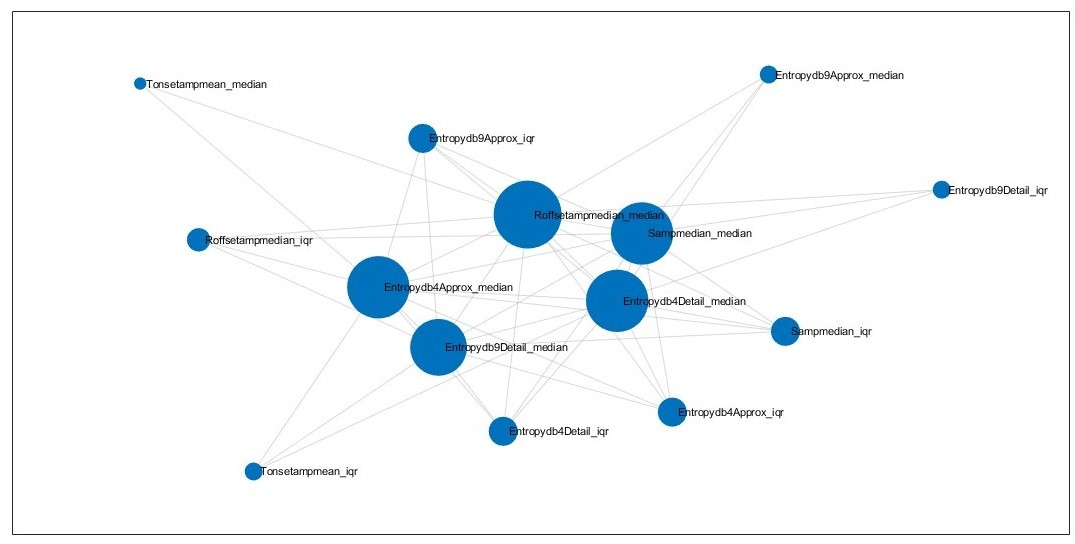
\includegraphics[width=1.0\textwidth]{map80.jpg}
    \caption{Network diagram of the pairs of features with more than 80\% correctly predicted observations.}
    \label{fig:map80}
\end{figure}



\subsection{Multiple Comparison Test}

To determine whether these features can distinguish pain from the lack of it in spite of the context, statistical analysis was performed through a multiple comparison test applied to both the baselines and to the pain phase. This was done for each participant first, using the original features that resulted in the selected ones, and then for the extracted features. Firstly, a one-way \ac{anova} was applied to the three groups. This test evaluates whether there are statistically significant differences between the means of each group. Afterwards, the Tukey-Kramer method, also known as the \ac{hsd} method, was performed as a post-hoc test to determine whether the differences detected by the \ac{anova} test are significant. This is done by taking the absolute value of the difference between pairs of means and dividing it by the standard error of the mean \cite{Nanda2021}. %The SE is in turn the square root of (variance divided by sample size)


Analysing each participant's data individually, regarding the median of the R offset amplitude, the means of the pain and baseline phases were different for 100\% of the participants, with 20\% of the baselines' means being coincident. For the median of the S amplitude, there was 93\% of successful pain and baselines' means distinction, where 43\% corresponded to similar means when comparing the baselines.
Lastly, the entropy of the approximation of the db4 and db9 wavelets acquired analogous results, with 80\% of the participants' pain and baselines' means being significantly different. 25\% of these participants' baselines 1 and 2 had similar means for both of these features. These results suggest that, for most participants, these features are successful in describing pain. Additionally, it's viable that the video watched by each participant has affected not only the entropy of the \ac{ecg} and the R offset, but mostly the amplitude of the S wave. In Figures \ref{fig:multcompR} to \ref{fig:multcomp9}, examples of this multiple comparison tests are displayed for each feature. 



\begin{figure}[htbp]
    \centering
    \begin{minipage}{0.49\textwidth}
        \centering
        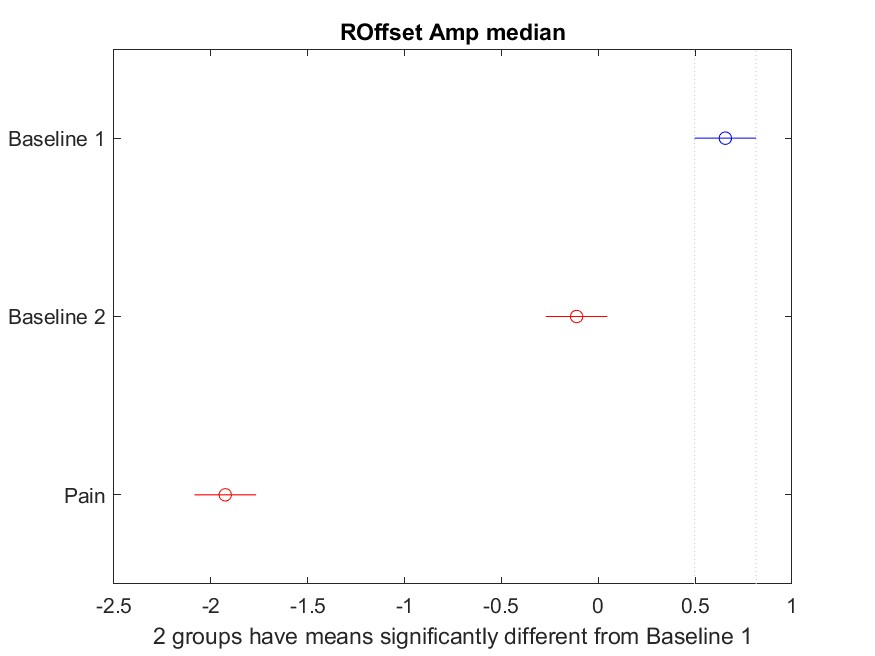
\includegraphics[width=6.8cm]{ROffset Amp median_part2.jpg}
        \caption{Multiple comparison test of the R offset amplitude for a participant's baselines and pain phase.}
        \label{fig:multcompR}
    \end{minipage}
    \hfill
    \begin{minipage}{0.49\textwidth}
        \centering
        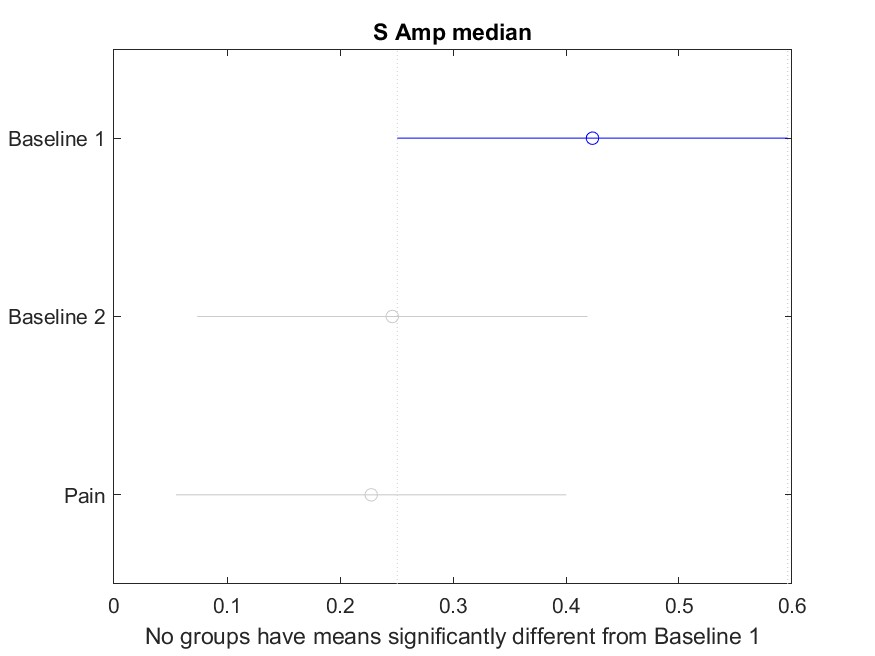
\includegraphics[width=6.8cm]{S Amp median_part2.jpg}
        \caption{Multiple comparison test of the S wave amplitude for a participant's baselines and pain phase.}
        \label{fig:multcompS}
    \end{minipage}
\end{figure}



\begin{figure}[htbp]
    \centering
    \begin{minipage}{0.49\textwidth}
        \centering
        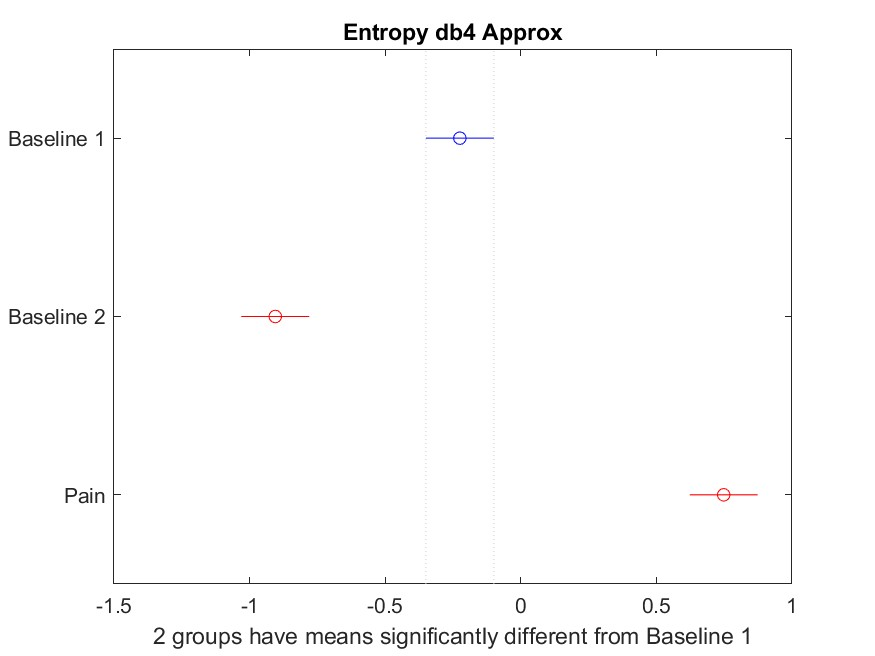
\includegraphics[width=6.8cm]{Entropy db4 Approx_part2.jpg}
        \caption{Multiple comparison test of the entropy of the db4 approximation for a participant's baselines and pain phase.}
        \label{fig:multcomp4}
    \end{minipage}
    \hfill
    \begin{minipage}{0.49\textwidth}
        \centering
        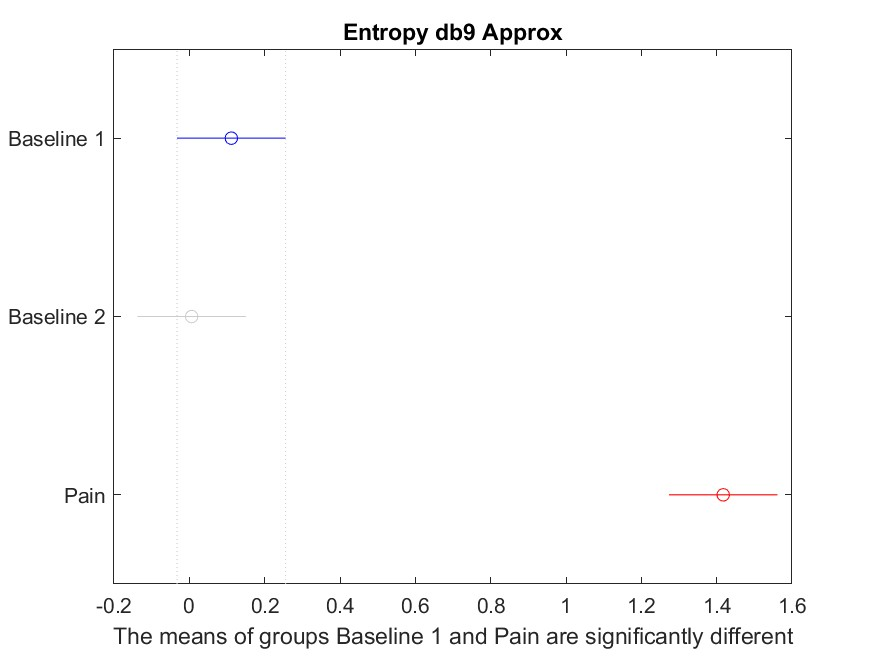
\includegraphics[width=6.8cm]{Entropy db9 Approx_part34.jpg}
        \caption{Multiple comparison test of the entropy of the db9 approximation for a participant's baselines and pain phase.}
        \label{fig:multcomp9}
    \end{minipage}
\end{figure}

\pagebreak

On the other hand, the result of this test for the selected extracted features is portrayed in Figure \ref{fig:five_images}. As can be seen, the baselines' means are significantly different from the pain phase's for all the selected features, which supports the idea that pain has an impact on both the S wave and entropy. 
Furthermore, the means of the baselines are similar in all the graphics, which means both can be used to describe pain. However, there’s a slight difference between the baselines for the amplitude of the S wave. This might be due to the visual stimulus having an impact on the ventricular polarization.




\begin{figure}[htbp]
    \centering
    % First row of 2 images
    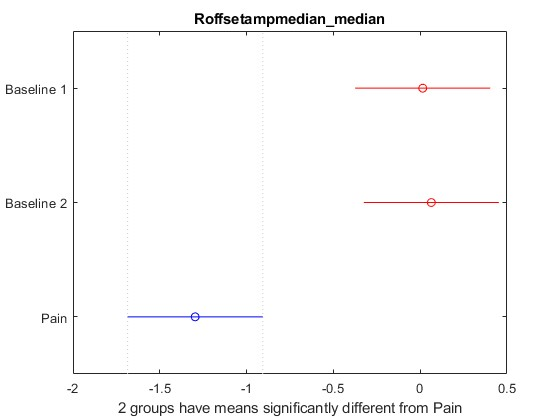
\includegraphics[width=0.49\linewidth]{multcompareR.jpg}
    \hfill
    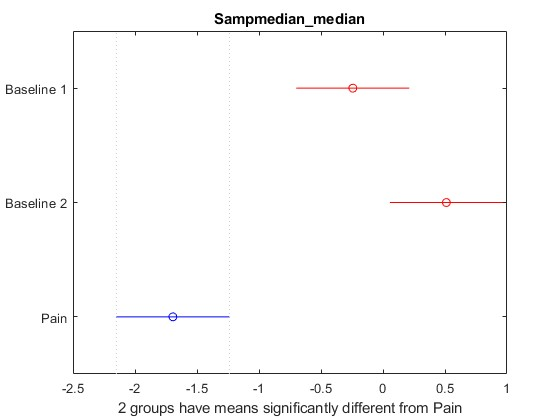
\includegraphics[width=0.49\linewidth]{multcompareS.jpg}
    \vspace{0.5em}  % space between rows
    % Second row of 2 images
    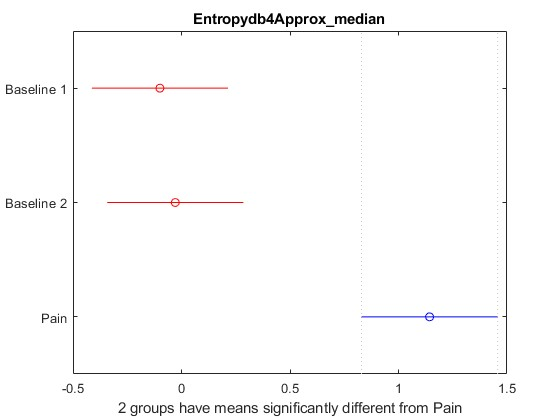
\includegraphics[width=0.49\linewidth]{multcompare4approx.jpg}
    \hfill
    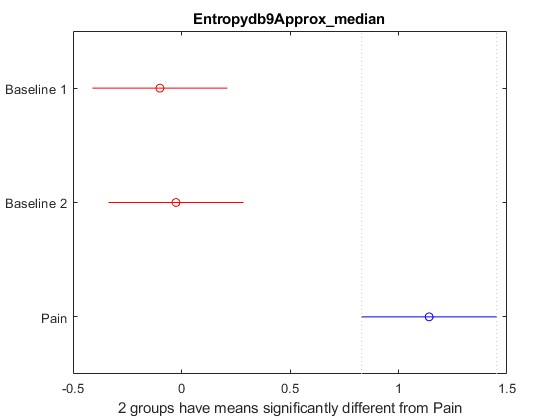
\includegraphics[width=0.49\linewidth]{multcompare9approx.jpg}
    \vspace{0.5em}  % space between rows
    \caption{Multiple comparison test (\ac{anova} + HSD) applied to both the baselines and to the pain phase, for each of the selected features.}
    \label{fig:five_images}
\end{figure}

\pagebreak 
\section{K-Nearest Neighbours}

In order to validate the results of this project, a Classification Learner algorithm, particularly, a \ac{knn} classifier was employed on the selected features. This classifier is widely used due to its simplicity and effectiveness but, for this project, it was chosen because of its classification technique's similarity to the clustering algorithm. \ac{knn} classification starts with the determination of the K-nearest neighbours, which is done by computing the distance between an unknown example $q$, that must be classified, and $x_i$ training samples. This distance is described by Equation \ref{eq:4}, which is a summation for all the features in $F$, with $w_f$ being the weight for each feature and $\delta$ a specific distance metric \cite{Cunningham2022}. Then, a majority voting is applied and $q$ is characterised as the class of the majority of its K-nearest neighbours \cite{Papanikolaou2021}.

\begin{equation} \label{eq:4}
d(q,x_i)=\sum_{f\epsilon F}^{}w_f\delta(q_f,x_{if})
\end{equation}



To create this classifier, MATLAB's Classification Learner app was used, along with the processed features from the aforementioned fifteen participants. For the distance metric, Euclidian distance was chosen. This metric is computed as the square root of the sum of squared differences between the elements of both vectors, according to Equation \ref{eq:4}.

\begin{equation} \label{eq:4}
\delta(x,y)=\sqrt{\sum_{i=1}^{n}(x_i-y_i)^2}
\end{equation}

The remaining hyperparameters were selected using Bayesian optimisation. The goal of this optimisation is to find the ideal combination of parameters that minimizes cross-validation loss. After performing a search with 30 iterations, the optimised parameters were selected and used in the model. These are portrayed in Table \ref{table:hyperparameters}. 

\begin{table}[h]
    \centering
    \captionsetup{justification=raggedright, singlelinecheck=false}
    \caption{Hyperparameters optimisation search range and results.}
    \renewcommand{\arraystretch}{1.2}

    \begingroup
    \hyphenpenalty=10000
    \exhyphenpenalty=10000
    \sloppy
    \begin{tabular}{@{}>{\RaggedRight\arraybackslash}p{4.3cm} >{\RaggedRight\arraybackslash}p{5.7cm} >{\RaggedRight\arraybackslash}p{4cm}@{}}
        \hline
        \textbf{Hyperparameters} & \textbf{Search Range} & \textbf{Optimised Values} \\
        \midrule
        Number of neighbours & 1-15 & 2 \\
        [1ex]
        Distance weight & Equal, Inverse, Squared inverse & Equal \\
        [1ex]
        Standardised & True, False & False \\
    \end{tabular}
    \endgroup
    \label{table:hyperparameters}
\end{table}    



Once the hyperparameters were selected, the model was trained using the fifteen participants' features as the training set. This was done through fivefold cross-validation, that uses one fifth of the data to evaluate the model in each iteration. Once the \ac{knn} model was complete, the processing pipeline was applied to the remaining 36 participants' data to create a training dataset. Then, the model was applied to this set, predicting whether a value had derived from the baseline or pain stimulation phase. To compare these predictions with the true values, a confusion matrix was plotted in Figure \ref{fig:confusiontest}. This allows for the computation of the following variables:

\begin{itemize}
   \item \textbf{\ac{tp}:} pain observations correctly predicted.
   \item \textbf{\ac{fp}:} pain observations incorrectly predicted.
   \item \textbf{\ac{tn}:} baseline observations correctly predicted.
   \item \textbf{\ac{fn}:} baseline observations incorrectly predicted.
 \end{itemize}

 \begin{figure}[h!]
    \centering
    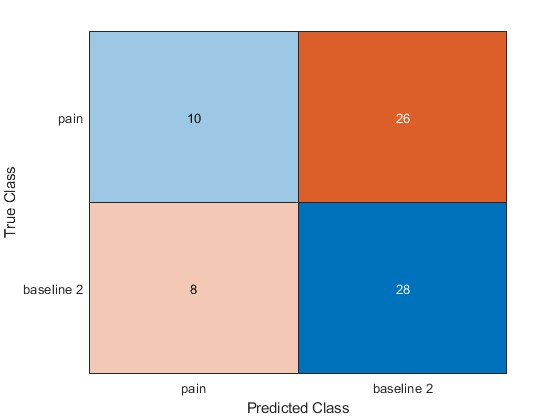
\includegraphics[width=0.7\textwidth]{confusion test.jpg}
    \caption{Confusion matrix for KNN model testing.}
    \label{fig:confusiontest}
\end{figure}

These variables can be used to calculate metrics for classification models' evaluation, such as sensitivity, precision, accuracy, and F-score. Sensitivity, also known as True Positive Rate, is obtained by dividing the number of \ac{tp} for the sum of \ac{tp} and \ac{fn}. On the other hand, specificity, or True Negative Rate, corresponds to the number of \ac{tn} divided by the sum of \ac{tn} and \ac{fp}. Meanwhile, precision is computed as the ratio between the \ac{tp} and the total number of pain predictions, while accuracy is computed as the sum of \ac{tp} and \ac{tn} divided by the total number of observations \cite{Vujovic2021}. 

\pagebreak

\begin{table}[h]
    \centering
    \captionsetup{justification=raggedright, singlelinecheck=false}
    \caption{Features for pain classification after data preparation procedures.}
    \renewcommand{\arraystretch}{1.2}

    \begingroup
    \hyphenpenalty=10000
    \exhyphenpenalty=10000
    \sloppy
    \begin{tabular}{@{}>{\RaggedRight\arraybackslash}p{4.5cm} >{\RaggedRight\arraybackslash}p{3.5cm}@{}}
        \hline
        \textbf{Evaluation Metric} & \textbf{Percentage} \\
        \midrule
        Sensitivity & 27.8\% \\
        [1ex]
        Specificity & 77.8\% \\
        [1ex]
        Precision & 55.6\% \\
        [1ex]
        Accuracy & 52.8\% \\
    \end{tabular}
    \endgroup
    \label{table:evaluationmetrics}
\end{table}

As shown in Table \ref{table:evaluationmetrics}, the \ac{knn} model achieved a low sensitivity of 27.8\%. This implies that the model was unsuccessful in correctly identifying true cases of pain, contesting the validity of these features for pain description. In contrast, the specificity was relatively high at 77.8\%, indicating that the model was more effective in correctly identifying the absence of pain. Additionally, an accuracy of 52.8\% was obtained, which indicates that approximately half of the predictions made on the test set were correct. Meanwhile, precision reached 55.6\%, suggesting that slightly more than half of the observations classified as pain were true positives. 